\documentclass{article}
\usepackage{amsmath}
\usepackage{amssymb}
\usepackage{amsfonts}
\usepackage{mathrsfs}
\usepackage{graphicx}
\usepackage{float}
\usepackage[margin=1in]{geometry}
\usepackage{tikz}
\usetikzlibrary{shapes.multipart, arrows.meta, positioning}
\tikzset{
    class/.style={
        rectangle split, 
        rectangle split parts=3, 
        draw, 
        align=left, 
        text width=4cm,
        font=\small
    },
    abstract/.style={
        class,
        font=\itshape
    },
    inheritance/.style={
        -{Triangle[open]}, 
        thick
    }
}
% Safety net: Common AI hallucinated commands for UML diagrams
\providecommand{\attribute}[1]{\textit{#1}}
\providecommand{\method}[1]{\texttt{#1}}
\providecommand{\classname}[1]{\textbf{#1}}
\begin{document}

\begin{figure}[h!]
\centering
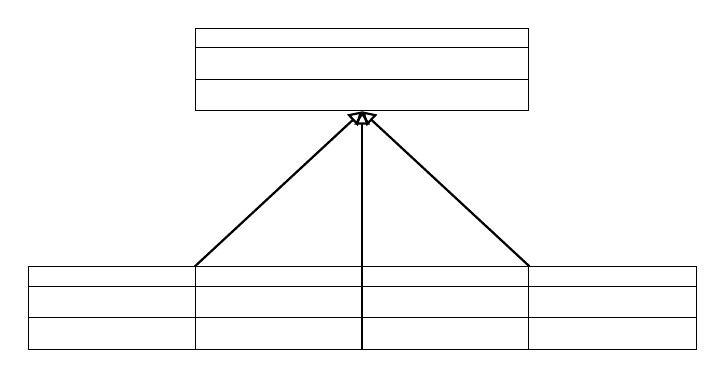
\begin{tikzpicture}
    % Nodes for classes
    \node (Transaction) [abstract={
        \textbf{Transaction}
    }{
        - accountNumber : Integer
    }{
        \textit{+ getAccountNumber()}\par \textit{+ execute()}
    }] {};

    \node (BalanceInquiry) [class={
        \textbf{BalanceInquiry}
    }{}{
        + execute()
    }] at ([yshift=-2.5cm]Transaction.south west) {}; % Position relative to Transaction
    \node (Withdrawal) [class={
        \textbf{Withdrawal}
    }{
        - amount : Double
    }{
        + execute()
    }] at ([yshift=-2.5cm]Transaction.south) {}; % Position relative to Transaction
    \node (Deposit) [class={
        \textbf{Deposit}
    }{
        - amount : Double
    }{
        + execute()
    }] at ([yshift=-2.5cm]Transaction.south east) {}; % Position relative to Transaction

    % Inheritance arrows
    \draw [inheritance] (BalanceInquiry.north) -- (Transaction.south);
    \draw [inheritance] (Withdrawal.north) -- (Transaction.south);
    \draw [inheritance] (Deposit.north) -- (Transaction.south);

\end{tikzpicture}
\caption{\textit{Figure 2 Class Diagram}}
\end{figure}

Your task is to write a java code by using Factory Design Pattern for the delegation of object creation to achieve loose coupling.

Note: You may make your own intuition about methods/functions.

\vspace{1em} % Add some space before the header

{\hrule height 0.4pt} % Rule above
\vspace{0.5em}
\noindent\textbf{Question \# 6: CLO-4} \hfill \textbf{Marks: [10] Time: [15 mins]}
\vspace{0.5em}
{\hrule height 0.4pt} % Rule below
\vspace{1em}

Singleton Design Pattern ensures that there is only one instance of a class and provides a global point of access to it. Consider the scenario of an ATM transaction given in \textbf{Question \# 5}and write a java code to restrict the creation of multiple instances of transaction class.

\vspace{1em} % Add some space before the header

{\hrule height 0.4pt} % Rule above
\vspace{0.5em}
\noindent\textbf{Question \# 7: CLO-5} \hfill \textbf{Marks: [10] Time: [15 mins]}
\vspace{0.5em}
{\hrule height 0.4pt} % Rule below
\vspace{1em}

Fire Alarming System: The owner of a large multi-stored building wants to have a computerized fire alarm system for his building. Smoke detectors and fire alarms would be placed in each room of the building. The fire alarm system would monitor the status of these smoke detectors. Whenever a fire condition is reported by any of the smoke detectors, the fire alarm system should determine the location at which the fire condition is reported by any of the smoke detectors, and then sound the alarms only in the neighboring locations. The fire alarm system should also flash an alarm message on the computer console.
\begin{itemize}
    \item Design an architecture based on an event-driven style.
\end{itemize}

\vspace{1em} % Add some space before the header

{\hrule height 0.4pt} % Rule above
\vspace{0.5em}
\noindent\textbf{Question \# 8: CLO-5} \hfill \textbf{Marks: [10] Time: [15 mins]}
\vspace{0.5em}
{\hrule height 0.4pt} % Rule below
\vspace{1em}

\begin{itemize}
    \item Discuss microservices architecture by comparing it with a monolithic architectural approach.
\end{itemize}

\vspace{2em} % More space before GOOD LUCK!
\centering\textbf{GOOD LUCK!}

\end{document}